% !TeX root = ./main.tex
\documentclass[main]{subfiles}
\begin{document}
\part*{Дифференциальная геометрия}
\chapter{Дифференциальная геометрия кривых}
\section{Понятие кривой} \marginpar{05.09.22}
Кривую можно задать множеством способов, например:
\begin{itemize}
    \item в декартовых координатах: $y = f(x)$
    \item в полярных координатах: $r = r(\phi)$
    \item неявным уравнением: $F(x,y) = 0$
\end{itemize}
но обычно её задают в параметрическом виде:
\[\begin{cases}
        x = x(t) \\
        y = y(t) \\
        z = z(t)
    \end{cases}\]
В таком случае кривая
\begin{itemize}
    \item в декартовых координатах принимает вид: $\displaystyle\begin{cases}
                  x = t \\
                  y = f(t)
              \end{cases}$
    \item в полярных координатах: $\displaystyle \begin{cases}
                  x = r(t) \cos t \\
                  y = r(t) \sin t
              \end{cases}$
    \item для неявных уравнений свои методы, т.к. не очень понятно как с ними работать
\end{itemize}

Например, для неявных уравнений существует следующая теорема:
\begin{theorem*}[О неявной функции]
    Если $F(x,y) = 0$ и $F(x_0, y_0) = 0$,
    а так же $\frac{\partial F}{\partial y}\rvert_{(x_0, y_0)} \neq 0$,
    $\frac{\partial F}{\partial x}, \frac{\partial F}{\partial y}$ существуют и непрерывны в окрестности $(x_0, y_0)$,
    тогда существует $f(x)$ в некоторой окрестности $x_0$, что $F(x, f(x)) =0$.
\end{theorem*}
\begin{example}
    Имеем стандартное уравнение окружности: $x^2 + y^2 -1 =0$.
    В окрестности большинства его точек можно выразить $y$ через $x$: $y = \pm \sqrt{1-x^2}$.
    Но это выражение перестает работать в точке $x=-1$ или $x=1$
    (то есть для любой другой точки, можно найти окрестность, такую что функция будет иметь конкретный знак, в то время как для $x= \pm 1$ такое сделать невозможно).
    Воспользуется теоремой выше, соблюдены почти все условия, кроме:
    \[\frac{\partial F}{\partial y} = 2y\rvert_{\substack{x = \pm 1\\ y=0}} = 0\]
    Соответственно, именно в этих точках найти искомую $f$ нельзя.
\end{example}

\subsection{Параметрическое задание кривой}
$\vf (t)$ - векторное уравнение. $\vf: [a,b] \to \R^3$.
Кривую определяет вектор-функция.

\begin{definition}[Вектор-функция]
    $\vf$ -- вектор-функция как выше.
    На протяжении всего курса предполагаем, что у функции необходимая нам гладкость.
\end{definition}

\begin{definition}[Предел вектор-функции]
    $\displaystyle \lim_{t \to t_0} \vf (t) = \vv$, если
    \[\forall \epsilon > 0 \ \exists \delta > 0 \ |t - t_0| < \delta \ |\vf(t) - \vv| < \epsilon\]
\end{definition}
\begin{propertylist}
    Везде считаем, что свойство выполнено, если существуют соответствующие пределы.
    \begin{enumerate}
        \item $\displaystyle \lim_{t \to t_0} ( \vf(t) \pm \vg (t))= \lim_{t \to t_0} \vf(t) \pm \lim_{t \to t_0} \vg (t) $
        \item $\displaystyle \lim_{t \to t_0} ( \vf(t) \vg (t))= \lim_{t \to t_0} \vf(t) \lim_{t \to t_0} \vg (t) $
        \item $\displaystyle \lim_{t \to t_0} ( \vf(t) \times \vg (t))= \lim_{t \to t_0} \vf(t) \times \lim_{t \to t_0} \vg (t) $
        \item Смешанное произведение аналогично
    \end{enumerate}
\end{propertylist}

\begin{definition}[Производная вектор-функции]
    \[\vf'(t)\rvert_{t=t_0} =  \lim_{t \to t_0} \frac{\vf(t) - \vf(t_0)}{t - t_0}\]
\end{definition}

\begin{propertylist}
    \

    \begin{enumerate}
        \item $\displaystyle (\vf \pm \vg)' = \vf' \pm \vg'$
        \item $\displaystyle (c\vf)' = c\vf'$
        \item $\displaystyle (\vf \vg)' = \vf'\vg + \vf \vg'$
        \item $\displaystyle (\vf \times \vg)' = \vf' \times \vg + \vf \times \vg'$
              \begin{proof}
                  \begin{multline*}
                      (\vf \times \vg)'\rvert_{t=t_0} = \lim_{t \to t_0} \frac{\vf(t) \times \vg(t) - \vf(t_0) \times \vg(t_0)}{t - t_0} = \\
                      \lim_{t \to t_0} \frac{\vf(t) \times \vg(t) - \vf(t_0) \times \vg(t) + \vf(t_0) \times \vg(t) - \vf(t_0) \times \vg(t_0)}{t - t_0} = \\
                      \lim_{t \to t_0} \frac{\vf(t) - \vf(t_0)}{t - t_0} \times \vg(t) + \lim_{t \to t_0} \vf(t_0) \times \frac{\vg(t) - \vg(t_0)}{t- t_0} = \\
                      \vf'(t_0) \times \vg(t_0) + \vf(t_0) \times \vg'(t_0)
                  \end{multline*}
              \end{proof}
        \item $\displaystyle (\vf,\vg,\vh)' = (\vf',\vg,\vh) + (\vf,\vg',\vh) + (\vf,\vg,\vh')$
              \begin{proof}
                  \begin{multline*}
                      (\vf,\vg,\vh)' = ((\vf \times \vg) \vh)' = (\vf \times \vg)' \vh + (\vf \times \vg) \vh'=\\
                      (\vf' \times \vg) \vh + (\vf \times \vg') \vh + (\vf \times \vg) \vh'
                  \end{multline*}
              \end{proof}
    \end{enumerate}
\end{propertylist}

В свойствах отсутствует деление, т.к. операция деления векторов не определена.
В вещественном анализе множество теорем доказывается с помощью следующей теоремы:
\begin{theorem*}[Лагранжа]
    Если $f(x)$ непрерывно дифференцируема на $[a,b]$, тогда существует $c \in [a,b] : f'(c) = \frac{f(b) - f(a)}{b-a}$.
\end{theorem*}
Для вектор-функций эта теорема, однако, не существует!


\begin{definition}[Интеграл вектор-функции]
    \[\int_a^b \vf(t) dt = \lim_{\max |\Delta_i t| \to 0} \sum_i \vf(\sigma_i) \Delta_i t.\]
\end{definition}
\begin{definition}[Кривая]
    Кривая -- образ $\vf(t)$.
    Кривая не пересекает саму себя, то есть $\vf(t_1) \neq \vf(t_2)$.
    $\vf(t)$ -- параметризация кривой.
    Параметризация регулярна, если $\vf'(t) \neq \vzero\ \forall t$.
\end{definition}
\begin{example}[Нерегулярная параметризация]
    $\displaystyle \begin{cases}
            x = t^2 \\
            y = t^3
        \end{cases}$ или $\vr(t) = (t^2, t^3)$ --
    полукубическая парабола. $y = x^{3/2}$ (плохо при $x<0$).
    \begin{center}
        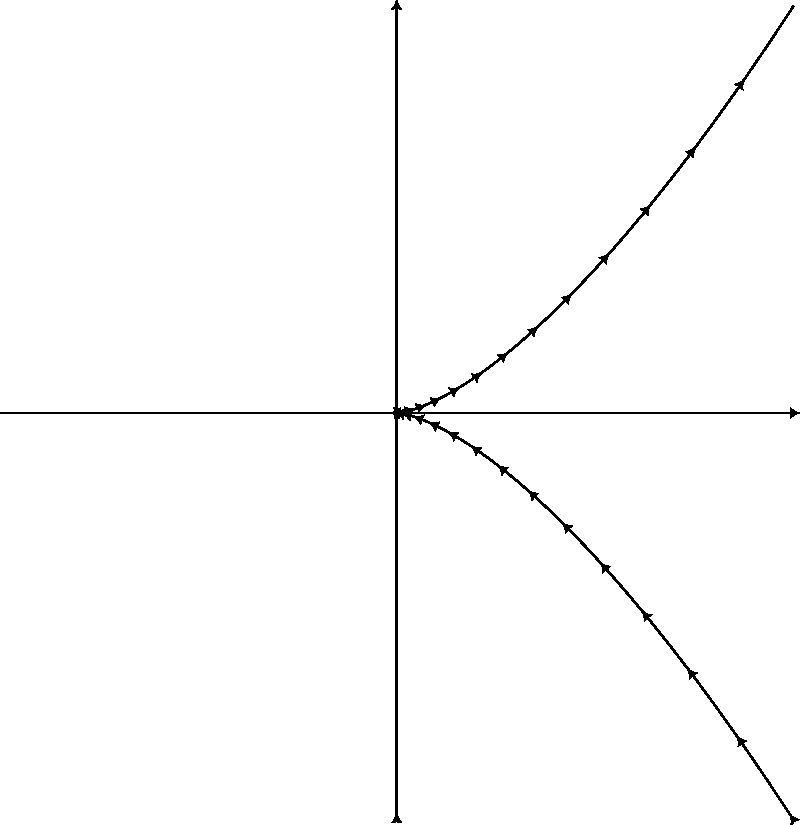
\includegraphics[width=0.5\linewidth]{semicubical_parabola.pdf}
    \end{center}

    $(0,0)$ -- точка излома (т.е. точка, в которой параметризация теряет регулярность).
\end{example}

\subsection{Перепараметризация}
Пусть $\phi: [a,b] \to [c,d]$, $\phi$ строго возрастает, $\phi(a) = c, \phi(b) = d$, также существует $\phi^{-1}$.
$\vf: [c,d] \to \R^3$, тогда $\vg \coloneqq \vf \circ \phi: [a,b] \to \R^3$.
В таком случае $\vg$ -- перепараметризация кривой и $\vf = \vg \circ \phi^{-1}$.

Если такая $\phi$ существует, то $\vf \sim \vg$ (эквивалентны).

Если образы $\vf(t)$ и $\vg(t)$ совпадают, кривые не самопересекаются,
а их параметризации регулярны, то существует такое $\phi$ и $\vf = \vg \circ \phi$.

\section{Длина кривой}
\begin{definition}[Длина кривой]
    $\vf: [a,b] \to \R^3$, $a = t_0 < t_1 < ... < t_n = b$, $\Delta_i t = t_i - t_{i-1}$.
    \[L \coloneqq \lim_{\max \Delta_i t \to 0} \sum_{i=1}^n |\vf(t_i) - \vf(t_{i-1})|\]
\end{definition}

\begin{definition}[Спрямляемая кривая]
    Прямая называется спрямляемой, если существует её длина.
\end{definition}
\begin{example}
    $y = \sin 1/x$  на $(0, 1]$ не спрямляемая.
    \begin{center}
        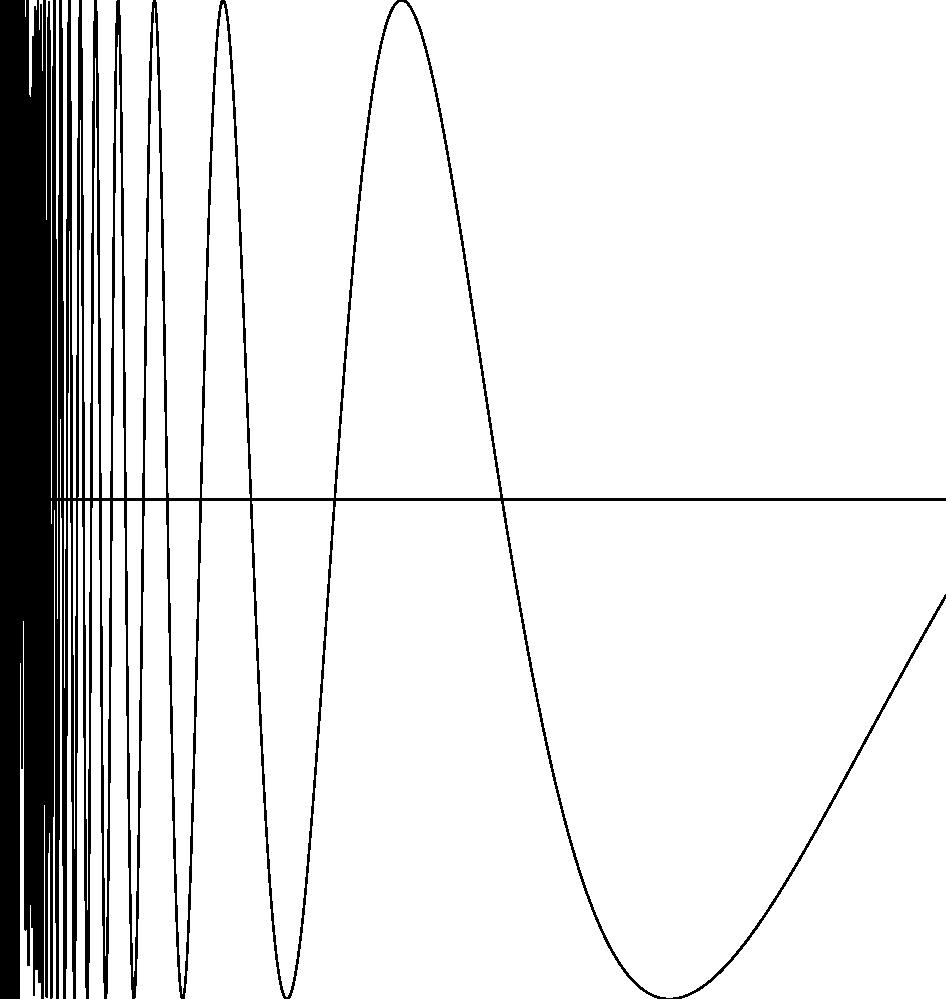
\includegraphics[width=0.5\linewidth]{sin_1_over_x.pdf}
    \end{center}
\end{example}
\begin{example}
    $y = \sqrt{x} \sin 1/x$, $y(0) = 0$, ее сумма оценивается $L \ge \sum_{n=1}^\infty \sqrt{\frac{1}{n}} = \infty$.
\end{example}
\begin{theorem}
    \[L = \int_a^b |\vf'(t)| dt \]
\end{theorem}
\begin{remark}
    $|\sum \vf_i| \le \sum |\vf_i|$, $||\vf| - |\vg|| \le |\vf - \vg|$, $|\int \vf dt| \le \int |\vf| dt$.
\end{remark}
\begin{proof}
    Хотим доказать:
    \[\left| \int_a^b |\vf'(t)| dt - \sum |\vf(t_i) - \vf(t_{i-1})|\right| \to 0\]
    оценим это:
    \begin{multline*}
        \left| \int_a^b |\vf'(t)| dt - \sum |\vf(t_i) - \vf(t_{i-1})|\right| = \\
        \left| \int_a^b |\vf'(t)| dt - \sum |\vf'(\sigma_i)| \Delta_i t  + \sum |\vf' (\sigma_i)| \Delta_i t - \sum |\vf(t_i) - \vf(t_{i-1})| \right| \\
        \le \left| \int_a^b |\vf'(t)| dt - \sum |\vf'(\sigma_i)| \Delta_i t \right|  +\\
        \left| \sum |\vf' (\sigma_i)| \Delta_i t - \sum |\vf(t_i) - \vf(t_{i-1})| \right|
    \end{multline*}
    $\left| \int_a^b |\vf'(t)| dt - \sum |\vf'(\sigma_i)| \Delta_i t \right| \to 0$ по определению интеграла.

    $\vf'$ непрерывная, значит равномерно непрерывна, тогда если
    $\forall \epsilon > 0\  \exists \delta > 0\  |x_1 - x_2| < \delta \implies |\vf(x_1) - \vf(x_2)| < \epsilon$.
    Выберем любое $\epsilon$ и зафиксируем $\delta$, удовлетворяющее мелкости разбиения и получим:
    \begin{multline*}
        \left| \sum |\vf' (\sigma_i)| \Delta_i t - \sum |\vf(t_i) - \vf(t_{i-1})| \right| =\\
        \left|\sum \int_{t_{i-1}}^{t_i} |\vf'(\sigma_i)|dt -  \sum \left|\int_{t_{i-1}}^{t_i} \vf'(t)dt\right|\right|
        \le \sum \int_{t_{i-1}}^{t_i} \left|\vf'(\sigma_i) - \vf'(t) \right|dt \\
        \le \sum \int_{t_{i-1}}^{t_i} \epsilon dt = \epsilon (b-a) \to 0
    \end{multline*}
\end{proof}

\newpage % It's a curse! Remove if something moves before this!
\marginpar{12.09.22}
Попытаемся понять как вычислять длину прямой в некоторых случаях:
\begin{itemize}
    \item в случае явного задания:
          \begin{gather*}
              \displaystyle \begin{cases}
                  x = t \\
                  y = f(t)
              \end{cases} \Leftrightarrow y = f(t) \\
              |(x',y')|  = \sqrt{1 + \vf'^2(t)} \implies
              L = \int_a^b\sqrt{1 + \vf'^2(t)} dt
          \end{gather*}
          К сожалению, такая формула мало применима, так как интегралы берутся редко.
    \item в случае параметрического задания:
          \begin{gather*}\begin{cases}
                  x = x(t) \\
                  y = y(t) \\
                  z = z(t)
              \end{cases} \implies
              L = \int_a^b \sqrt{x'^2 + y'^2 +z'^2} dt
          \end{gather*}
    \item в случае полярных координат:
          \begin{gather*}
              r = r(\phi) \Leftrightarrow \begin{cases}
                  x = r(\phi) \cos \phi \\
                  y = r(\phi) \sin \phi
              \end{cases} \implies
              \begin{cases}
                  x' = r' \cos \phi -r \sin \phi \\
                  y' = r' \sin \phi + r \cos \phi
              \end{cases} \\
              \begin{multlined}
                  x'^2 + y'^2 = (r' \cos \phi -r \sin \phi)^2 + (r' \sin \phi + r \cos \phi)^2 = \\
                  r'^2\cos^2 \phi - 2rr'\sin \phi \cos \phi + r^2 \sin^2 \phi +\\
                  r'^2 \sin^2\phi + 2rr' \sin \phi \cos \phi + r^2 \cos^2 \phi = \\
                  r'^2 + r^2
              \end{multlined}\\
              L = \int_a^b \sqrt{x'^2 + y'^2} d\phi  = \int_a^b \sqrt{r'^2 + r^2}d \phi
          \end{gather*}
\end{itemize}

\section{Касательный вектор}
\begin{lemma}\label{dfoc:very_important_lemma}
    Если $|\vf(t)| = const$, то $\vf'(t) \perp \vf(t)$.
\end{lemma}
\begin{proof}
    Из $\vf'(t) \perp \vf(t)$ получаем: $ (\vf'(t), \vf(t)) = 0\ \forall t$.
    Возьмем производную скалярного квадрата и получим:
    \[(\vf(t), \vf(t))' = 2(\vf'(t), \vf(t)) = 0 = |\vf(t)|^{2'}\]
    Тогда, $|\vf(t)| = const$.
\end{proof}
\begin{definition}[Касательный вектор]
    $\vf'(t_0)$ называется касательным вектором к кривой в точке $t_0$.
    Прямая, на которой лежит $\vf'(t)$ -- касательная прямая.
\end{definition}
\begin{theorem}
    Касательная прямая не зависит от параметризации, если она регулярна.
\end{theorem}
\begin{proof}
    $\phi$ -- скалярная функция, $\vf(t)$ -- вектор-функция.
    Также $\vf(\phi(t)) = \vg(t)$.
    $\vf'(t)$, $\vg'(t) = \vf'(\phi(t)) \phi'(t)$ -- касательные векторы $\vf$ и $\vg$ соответственно.
    Обозначим $\tau = \phi(t)$.
    $\vf'(t)$ и $\vg'(t)$ отличаются друг от друга на скаляр,
    тогда $\vf'(\tau) \parallel \vg'(t)$.
    Следовательно, при перепараметризации касательный вектор будет параллелен предыдущему, значит касательная прямая инвариантно определена.
\end{proof}
\begin{remark}
    Регулярная параметризация -- это параметризации для которой в любой точке существует касательная прямая.
\end{remark}
\begin{definition}[Натуральная параметризация]
    Параметризация $\vf(t)$ называется натуральной, если $|\vf'(t)| \equiv 1\ \forall t$.
\end{definition}
По сути, мы идем по кривой с единичной скоростью.
Но пока не ясно существует и единственна ли натуральная параметризация.
\begin{proof}
    Проверить единственность достаточно просто: $\vg(t) = \vf(\phi(t))$, $\phi(t) = \tau$
    \[|\vg'(t)| = |\vf'(\tau)| |\phi(t)| \implies |\phi'(t)| = 1\]
    тогда $\phi = t + t_0$ (с точностью до выбора начального момента времени).
\end{proof}

\begin{theorem}
    Натуральная параметризация существует.
\end{theorem}
\begin{proof}
    Вспомним про длину кривой.
    Глобальная идея: параметризация говорит сколько мы проходим по кривой за данное время;
    чтобы перейти к натуральной параметризации мы откажемся от стандартного времени,
    и скажем, что новое время это тот участок кривой, за которое мы его проходим, или
    единичное расстояние мы проходим за единичное время, значит параметр времени -- это участок дуги.

    Реализуем эту идею:
    \[s = \int_{t_0}^t |\vf'(\tau)| d\tau\]
    $s$ -- искомый натуральный параметр.
    Будем считать $t - t_0$ временем.
    Обозначим $s = \phi(t)$:
    \[\phi(t) = \int_{t_0}^t |\vf'(\tau)| d\tau\]
    Заметим, что $\phi(t)$ возрастает и непрерывна.
    Значит существует $t = \phi^{-1}(s)  = \psi(s)$.
    Тогда $\vf(t) = \vf(\psi(s))$ должна быть натуральной параметризацией.

    Теперь докажем, что $\vf(\psi(s))$ есть натуральная параметризация.
    Хотим убедиться, что
    \[\left| \frac{d \vf(\psi(s))}{ds}\right| = 1.\]
    Для этого
    \begin{gather*}
        \psi'(s) = \frac{1}{\phi'(t(s))} = \frac{1}{|\vf'(t)|}\\
        \frac{d}{ds}\vf(\psi(s)) = \vf'(\psi(s)) \psi'(s) = \frac{\vf'(t)}{|\vf'(t)|}\\
        \left| \frac{\vf'(t)}{|\vf'(t)|} \right| = 1
    \end{gather*}
\end{proof}

\section{Реп\'ер Френ\'е}

Есть кривая и $\vf(s)$ -- ее натуральная параметризация, тогда $\vv(s)$ -- ее касательный вектор.
$|\vv(s)| = 1$.
Тогда $\vv'(s) \perp \vv(s)$ по лемме \ref{dfoc:very_important_lemma}.
\begin{definition}[Кривизна кривой]
    Определим $\vn(s)$: $\vn(s) \upuparrows \vv'(s)$, $|\vn(s)| = 1$,
    такой $\vn$ -- вектор главной нормали.
    \[k = \frac{\vv ' (s)}{\vn} \Leftrightarrow \vv' = k \vn\]
    Такая $k$ -- кривизна кривой.
    А выражение $\vv' = k \vn$ называется первой формулой Френе.
\end{definition}
\begin{remark}
    $k \ge 0$.
\end{remark}
\begin{remark}
    $\vn$ -- не везде определен, необходима бирегулярность.
\end{remark}

\begin{definition}
    Кривая называется бирегулярной, если $\vf''(t) \not\parallel \vf'(t)$ для любой параметризации.
    Или, если $\vv'(s) \neq 0$ для натуральной параметризации.
    Или $\vn$ корректно определен.
    (почему они эквивалентны -- вопрос будущего)
\end{definition}

По умолчанию считаем, что все кривые бирегулярны.

У нас есть вектор $\vv$ и перпендикулярный ему $\vn$.
Они единичные, хотим превратить их в базис пространства.
Для этого построим вектор $\vb$ перпендикулярный им обоим и тоже единичный.
\begin{center}
    \import{figures/}{binormal_vector.pdf_tex}
\end{center}

\begin{definition}[Вектор бинормали]
    \[\vb \coloneqq \vv \times \vn\]
    Правая тройка $(\vv,\vn, \vb$) -- репер Френе.
\end{definition}

Изучим $\vb'$:
$\vb'(s) \perp \vb(s)$ из леммы \ref{dfoc:very_important_lemma},
также $\vb' \perp \vv$. Почему?
\[\vb' = (\vv \times \vn)' = \vv' \times \vn + \vv\times \vn' = 0 + \vv\times \vn' \perp \vv\]
Таким образом, $\vb' \parallel \vn$ и $\vb' = -\kappa \vn$ -- вторая формула Френе.
\begin{definition}[Кручение кривой]
    $\kappa$, определенная выше -- кручение кривой.
\end{definition}

Изучим $\vn$:
\[\vn' = (\vb \times \vv)' = \vb' \times \vv + \vb \times \vv' = -\kappa \vn \times \vv + \vb \times k\vn = \kappa\vb - k\vv\]
получили третью формулу Френе.
\begin{definition}[Формулы Френе]
    \[
        \begin{array}{cccc}
            \toprule
                 & \vv & \vn     & \vb    \\ \midrule
            \vv' & 0   & k       & 0      \\ \midrule
            \vn' & -k  & 0       & \kappa \\ \midrule
            \vb' & 0   & -\kappa & 0      \\
            \bottomrule
        \end{array}
    \]
    Производная везде берется по натуральному параметру.
\end{definition}
\begin{definition}
    Плоскость $(\vn, \vb)$ -- нормальная плоскость кривой.
    Плоскость $(\vv, \vn)$ -- соприкасающаяся плоскость кривой.
    Плоскость $(\vv, \vb)$ -- спрямляющая плоскость кривой.
\end{definition}

Вопрос: а как это посчитать?
\begin{example}
    Есть окружность:
    \[\begin{cases}
            x = R \cos t \\
            y = R \sin t \\
            z = 0
        \end{cases}\]
    Хотим найти натуральную параметризацию:
    сейчас мы проходим окружность за время $2\pi$, наверное нужно проходить окружность за время $2\pi R$.
    Тогда получим:
    \[\begin{cases}
            x = R\cos (t/R)  \\
            y = R \sin (t/R) \\
            z = 0
        \end{cases}
        \implies
        \begin{cases}
            x' = - \sin (t/R) \\
            y' = \cos (t/R)
        \end{cases}\]
\end{example}

\section{Соприкасающаяся плоскость}\marginpar{19.09.22}
В натуральной параметризации $\vv = \vf'$ и $\vn = \vf''/k$.
Тогда плоскость $\langle \vf', \vf''\rangle$ -- соприкасающаяся плоскость для натуральной параметризации.

А что будет в случае не натуральной параметризации?
Посмотрим, что в таком случае происходит с вектором $\vf''$, будет ли он перпендикулярен $\vf'$?
Нет, не будет, потому что, если вектор $\vf'' \perp \vf'$, то $|\vf'| = const$
и параметризация почти натуральная, в том смысле, что наша скорость постоянная, но возможно не единичная.
Вывод: в обычной ситуации $\vf''$ не перпендикулярен $\vf'$, однако плоскость в которой он лежит не меняется.

% TODO: Выяснить понадобится ли часть про центростремительное и тангенциальное ускорения.
\begin{theorem}
    Плоскость $\langle \vf', \vf''\rangle$ не зависит от параметризации.
\end{theorem}
\begin{proof}
    Пусть $\vf(t) = \vg(s)$, где $s$ не обязательно натуральный параметр и $s = \phi(t)$, тогда $\vg(\phi(t)) = \vf(t)$.
    Уже доказано, что $\vf' \parallel \vg'$.
    Теперь выясним, что
    \begin{multline*}
        \vf''(t) = (\vg(\phi(t)))'' = (\vg'(\phi(t)) \phi'(t))' = \\
        \vg''(\phi(t)) \phi'^2(t) + \vg'(\phi(t)) \phi''(t) \in \langle \vg', \vg''\rangle
    \end{multline*}
\end{proof}

\begin{theorem}
    Есть регулярная параметризация $\vf(t)$,
    $\delta(t)$ -- расстояние от $\vf(t)$ до касательной в точке $\vf(t_0)$.
    \begin{center}
        \import{figures/}{approximation1.pdf_tex}
    \end{center}
    \[\lim_{t \to t_0} \frac{\delta}{|\vf(t) - \vf(t_0)|} = 0.\]
    Такой $\lim = 0$ тогда и только тогда, когда касательная прямая.
\end{theorem}
\begin{proof}
    Выберем удобную для нас координатную систему:
    \begin{itemize}
        \item $\vf(t_0) = (0,0,0)$
        \item $t_0 = 0$
        \item Касательная прямая -- прямая $OX$.
              Тогда $\vf(0) = (a,0,0)$.
    \end{itemize}
    Пусть $\vf(t) = (f_1(t), f_2(t), f_3(t))$, выясним что такое $\delta$.
    \[\delta = \sqrt{f_2^2(t) + f_3^2(t)}\]
    Разложим $f_1$ по Тейлору:
    \begin{gather*}
        f_1(t) = f_1(0) + f_1'(0)t + o(|\vf(t) - \vf(t_0)|) = at + o(t)
        \intertext{На малом промежутке $|\vf(t) - \vf(t_0)| \approx t$. Аналогично с $f_2, f_3$:}
        f_2 (t) = f_2(0) + f_2'(0)t+o(t) = o(t)\\
        f_3 (t) = o(t)
    \end{gather*}
    Отсюда, $\delta(t) = o(t)$ и
    \[\lim_{t \to 0} \frac{\delta(t)}{t} = 0\]
    А так же
    \[\lim_{t \to 0} \frac{|\vf(t) - \vf(0)|}{t} = |\vf'(0)|\]

    Обратное доказательство -- упражнение.
    (Hint: если $\delta$ -- расстояние от данной точки до любой прямой, кроме $OX$,
    то в формуле для $\delta$ появится слагаемое $f_1^2(t)$)
\end{proof}

% Здесь умирает звук в записи => снижается качество пояснений.
\begin{theorem}
    Пусть $\vf(t)$ -- бирегулярная параметризация.
    $\delta$ -- расстояние от $\vf(t)$ до плоскости $\alpha$.
    \begin{center}
        \import{figures/}{approximation2.pdf_tex}
    \end{center}
    \[\lim_{t \to t_0} \frac{\delta}{t^2} = 0 \left( \lim_{t \to t_0} \frac{\delta}{|\vf(t) - \vf(t_0)|^2} = 0 \right)\]
    Такой $\lim = 0 \Leftrightarrow \alpha$ -- соприкасающаяся плоскость.
\end{theorem}
\begin{proof}
    Введем удобную систему координат:
    \begin{enumerate}
        \item $t_0 = 0$
        \item $\vf(0) = (0,0,0)$
        \item $\vf'(0) = (a,0,0)$ и $\vf''(0) = (b,c,0)$
    \end{enumerate}
    Тогда соприкасающаяся плоскость, должна быть плоскостью $z=0$. Докажем это.

    Запишем вектор-функцию в координатах: $\vf(t) = (f_1(t), f_2(t), f_3(t))$.
    Пусть плоскость $\alpha$ задана уравнением $Ax+By+Cz+D = 0$ и $A^2 + B^2 + C^2 = 1$.
    Подсчитаем $\delta$ используя разложение по Тейлору:
    \begin{multline*}
        \delta = |Af_1(t) + Bf_2(t) + Cf_3(t) + D| =\\
        \left| A \left(f_1(0) + f_1'(0)t + \frac{f_1''(0)}{2}t^2 + o(t^2)\right) + \right.\\
        B \left(f_2(0) + f_2'(0)t + \frac{f_2''(0)}{2}t^2 + o(t^2)\right) + \\
        \left. C \left(f_3(0) + f_3'(0)t + \frac{f_3''(0)}{2}t^2 + o(t^2)\right) + D \right| = \\
        \left| Aat + \frac{Ab}{2} t^2 + \frac{Bc}{2}t^2 + D + o(t^2) \right|
    \end{multline*}
    Теперь хотим выяснить чему равносильно $\delta = o(t^2)$.
    \[\begin{cases}
            Aa = 0 \\
            Bc = 0 \\
            D = 0  \\
        \end{cases}\]
    При этом $a \neq 0$, т.к. это единственная ненулевая координата касательного вектора, она не может быть нулем.
    И $c \neq 0$, иначе $\vf''$ коллинеарно $\vf'$. Тогда
    \[\begin{cases}
            A = 0 \\
            B = 0 \\
            D = 0
        \end{cases}\]
    и $\alpha$ имеет единственно возможное уравнение $z = 0$.
\end{proof}

Посмотрим как задаются все эти плоскости в координатах.
Пусть
\[\vf(t) = (f_1(t), f_2(t), f_3(t))\]
и $\vf$ не натуральная параметризация (т.к. к натуральной параметризации тяжело перейти).
\[\vf'(t) = (f_1',f_2',f_3')\]

Построим нормальную плоскость:
\[f_1'(t_0)(x - f_1(t_0)) + f_2'(t_0)(y - f_2(t_0)) + f_3(t_0)(z - f_3(t_0)) = 0\]

Построим соприкасающуюся плоскость:
для этого найдем вектор главной нормали
\[\vn = \vf' \times \vf'' = (f_2'f_3'' - f_3'f_2'',f_3'f_1'' - f_1'f_3'', f_1'f_2'' - f_2'f_1'')\]
\begin{center}
    \import{figures/}{main_normal_vector.pdf_tex}
\end{center}
и уравнение плоскости
\[(f_2'f_3'' - f_3'f_2'')(x - f_1) + (f_3'f_1'' - f_1'f_3'')(y - f_2) + (f_1'f_2'' - f_2'f_1'')(z - f_3) = 0\]

Построение спрямляющей плоскости опущено в виду громоздкости выкладок.

\section{Вычисление кривизны и кручения}

В натуральной параметризации $\vf(s_0) = |\vf''(s_0)|$.
\begin{theorem}
    $k \equiv 0 \Leftrightarrow$ кривая является частью прямой.
\end{theorem}
\begin{proof}
    В натуральной параметризации $k=0$ равносильно $\vf''(t) = 0$,
    а это равносильно тому, что $\vf(t) = \vu t + \vv$, где $\vu$ и $\vv = const$.
\end{proof}
\begin{theorem}
    Для любой регулярной параметризации
    \[k = \frac{|\vf'(t) \times \vf''(t)|}{|\vf'(t)|^3}.\]
\end{theorem}
\begin{proof}
    Пусть $\vg(s)$ -- натуральная параметризация, а $\vf(t)$ любая другая параметризация.
    \[s = \phi(t) = \int_{t_0}^t |\vf'(\tau)| d\tau\]
    Тогда связь между ними: $\vf(t) = \vg(\phi(t))$.
    И существует $\psi(s) = t$ -- обратная функция и $\vg(s) = \vf(\psi(s))$.

    Пусть $\vu \in \langle \vf', \vf'' \rangle$
    \begin{center}
        \import{figures/}{proj_n-u.pdf_tex}
    \end{center}
    \[|\proj_\vn u| = \frac{|\vf' \times \vu|}{|\vf'|}\]

    Вычислим $k$:
    \begin{multline*}
        k = |\vg''(s)| = |(\vf(\psi(s)))''| = \\
        | \vf''(\psi(s)) \psi'^2(s) + \vf'(\psi(s)) \psi''(s)| = \\
        \proj_\vn (\vf''(\psi(s)) \psi'^2(s) + \vf'(\psi(s)) \psi''(s))
    \end{multline*}
    Пусть
    \begin{gather*}
        \vu = \vf''(\psi(s)) \psi'^2(s) + \vf'(\psi(s)) \psi''(s)\\
        \vf' \times \vu = \vf' \times \vf'' \psi'^2 + 0\\
        \psi'(s) = \frac{1}{\phi'(t)} = \frac{1}{|\vf'(t)|}
        \intertext{тогда}
        \frac{|\vf' \times \vu|}{|\vf'|} = \frac{|\vf' \times \vf''|}{|\vf'|}\psi'^2(s) = \frac{|\vf' \times \vf''|}{|\vf'|^3}
    \end{gather*}
\end{proof}

Если $\vf = (f_1, f_2, f_3)$, то
\[k = \frac{\sqrt{(f_2'f_3'' - f_3' f_2'')^2 + (f_3'f_1'' - f_1' f_3'')^2 + (f_1'f_2'' - f_2' f_1'')^2}}{(f_1^2 + f_2^2 + f_3^2)^{3/2}}\]
В случае плоских кривых ($f_3 = 0$):
\[k = \frac{|f_1'f_2'' - f_2' f_1''|}{(f_1^2 + f_2^2)^{3/2}}\]
При явном задании
\begin{gather*}
    y = f(x) \quad \begin{cases}
        x = f_1 = t \\
        y = f_2 = f(t)
    \end{cases}\\
    k = \frac{|f''|}{(1+ f'^2)^{3/2}}
\end{gather*}
В полярных координатах
\begin{gather*}
    r = r(\phi) \quad \begin{cases}
        f_1 = x = r \cos \phi \\
        f_2 = y = r \sin \phi
    \end{cases}\\
    |f'| = \sqrt{r^2 + r'^2} = \sqrt{f_1'^2 + f_2'^2}\\
    \begin{cases}
        f_1' = r' \cos \phi - r \sin \phi \\
        f_2' = r' \sin \phi + r \cos \phi
    \end{cases}\\
    \begin{cases}
        f_1'' = r'' \cos \phi - 2 r' \sin \phi - r \cos \phi \\
        f_2'' = r'' \sin \phi + 2 r' \cos \phi - r \sin \phi
    \end{cases}
\end{gather*}
Чему равно $|f_1'f_2'' - f_2' f_1''|$ -- упражнение.

\begin{theorem}
    Кривая плоская тогда и только тогда, когда ее $\kappa = 0$.
\end{theorem}\marginpar{26.09.22}
\begin{proof}
    Вспомним, что $\vb' = - \kappa \vn$ в натуральной параметризации.
    Тогда $\kappa = 0 \Leftrightarrow \vb' = 0 \Leftrightarrow \vb = const \Leftrightarrow$ соприкасающаяся плоскость $= const$.

    Если соприкасающаяся плоскость постоянная, то кривая лежит в ней.
    Докажем это.

    Ориентируем систему так, чтобы $\vb = (0,0,1)$.
    Кривая в натуральной параметризации имеет уравнение $\vg(s) = (g_1(s), g_2(s), g_3(s))$.
    И мы хотим доказать, что $g_3(s) = 0$.
    Рассмотрим вектор $\vb$:
    \[\vb = \frac{\vg' \times \vg''}{k}\]
    (Напоминание: в натуральной параметризации $\vv = \vg'$, $k\vn = \vv' = \vg''$, $\vb = \vv \times \vn$)
    \begin{gather*}
        \vg' \times \vg'' = (\underbrace{g_2' g_3'' - g_3'g_2''}_{=0}, \underbrace{g_3'g_1'' - g_1' g_3''}_{=0}, \underbrace{g_1'g_2'' - g_2' g_1''}_{\neq 0})
        \intertext{Получим систему:}
        \begin{cases}
            g_2' g_3'' - g_3'  g_2'' = 0              \\
            g_1' g_3'' - g_1'' g_3' = 0 & |\cdot g_2'
        \end{cases} \implies\\
        g_1'g_3' g_2'' - g_1'' g_3' g_2' = 0 \\
        g_3' (g_1' g_2'' - g_1'' g_2') = 0 \implies g_3' = 0\ \forall s \implies g_3 = const
    \end{gather*}
    значит третья координата кривой всегда одна и та же, а значит кривая лежит в плоскости $z = g_3 = const$.
\end{proof}

\begin{theorem}
    В натуральной параметризации
    \[\kappa = \frac{(\vg', \vg'', \vg''')}{k^2}.\]
\end{theorem}
\begin{proof}
    По формулам Френе
    \[\vb' = - \kappa \vn = - \kappa \frac{\vg'' }{k}\]
    при этом
    \[\vb = \frac{\vg' \times \vg''}{k}\]
    тогда
    \begin{align*}
        \vb' & = \left(\frac{\vg' \times \vg''}{k}\right)' =                                          \\
             & = \frac{(\vg'' \times \vg'') k + (\vg' \times \vg''')k - k'(\vg' \times \vg'')}{k^2} = \\
             & = -\kappa \frac{\vg''}{k}
    \end{align*}
    Посмотрим, чем являются производные $\vg$:
    \begin{gather*}
        \vg' = \vv\\
        \vg'' = \vv' = k \vn\\
        \vg''' = k'\vn + k\vn' = k'\vn + k(-k\vv + \kappa \vb) = k' \vn - k^2 \vv + k \kappa \vb\\
        \vg' \times \vg'' = \vv \times k \vn = k \vb
    \end{gather*}
    теперь посчитаем такое выражение:
    \begin{gather*}
        (\vg' \times \vg'') \cdot \vg''' = k \cdot k \kappa
        \intertext{итого получаем}
        \kappa = \frac{(\vg',\vg'' \vg''')}{k^2}
    \end{gather*}
\end{proof}
\begin{theorem}
    Для любой параметризации:
    \[\kappa = \frac{(\vf',\vf'', \vf''')}{|\vf' \times \vf''|^2}.\]
\end{theorem}
\begin{proof}
    Введем
    \[s = \int_{t_0}^t  |\vf'(\tau)| d\tau = \phi(t)\]
    -- натуральный параметр.

    Пусть $t = \psi(s)$, тогда $\vg(s) = \vf(t) = \vf(\psi(s))$ и
    $\psi'(s) = 1/\phi'(t) = 1/|\vf'(t)|$.
    Рассмотрим производные $\vg$:
    \begin{gather*}
        \vg'(t) = \vf'(t) \psi'(s) = \frac{\vf'}{|\vf'|}\\
        \vg'' = \vf'' \psi'^2 + \vf' \psi''\\
        \vg''' = \vf''' \psi'^3 + 3\vf''\psi'\psi'' + \vf' \psi'''
        \intertext{по свойствам смешаного произведения, все коллинеарные слагаемые можно записать один раз}
        (\vg', \vg'', \vg''') = (\vf'\psi', \vf'' \psi'^2, \vf''' \psi'^3 )
        = \psi'^6 (\vf', \vf'', \vf''')\\
        \kappa = \frac{(\vg', \vg'', \vg'')}{k^2} = \frac{(\vf', \vf'', \vf''')}{|\vf'|^6} \cdot \frac{|\vf'|^6}{|\vf' \times \vf''|^2}
    \end{gather*}
\end{proof}

\section{Натуральные уравнения кривой}

Есть кривая в натуральной параметризации.
Знаем $k(s)$ и $\kappa(s)$.
Верно ли, что существует ровно одна кривая, что эти функции являются ее кривизной и кручением?
Единственность точно верно, с существованием -- не всегда, $k$ должно быть положительно.

\begin{theorem}
    Если $\vg_1(s)$ и $\vg_2(s)$ -- кривые с одинаковыми $k$ и $\kappa$, тогда они отличаются друг от друга движением.
\end{theorem}
\begin{proof}
    В точке $s_0$ состыкуем реперы Френе.
    $(\vv_1(s), \vn_1(s), \vb_1(s))$ -- репер Френе для $\vg_1$.
    Аналогично, $(\vv_2(s), \vn_2(s), \vb_2(s))$ -- репер Френе для $\vg_2$.

    Что означает <<состыкуем>>?
    \begin{gather*}
        \vv_1 (s_0) = \vv_2(s_0)\\
        \vn_1 (s_0) = \vn_2(s_0)\\
        \vb_1 (s_0) = \vv_2(s_0)
    \end{gather*}

    Заведем скалярную функцию
    \[h(s) = \vv_1(s) \vv_2(s) + \vn_1(s) \vn_2(s) + \vb_1(s) \vb_2(s)\]
    заметим, что
    \begin{itemize}
        \item $h(s_0) = 3$
        \item $h(s) \le 3$ и $h(s) = 3 \Leftrightarrow \vv_1 = \vv_2, \vn_1 = \vn_2, \vb_1 = \vb_2$
    \end{itemize}
    Как доказать, что скалярная функция равна константе во всех точках, если мы знаем, что она равна константе в одной точке?
    Достаточно взять производную и показать, что она ноль.
    Возьмем производную $h$:
    \begin{multline*}
        h'(s) = \vv_1' \vv_2 + \vv_1 \vv_2' + \vn_1' \vn_2 + \vn_1 \vn_2' + \vb_1' \vb_2 + \vb_1 \vb_2' = \\
        = k \vn_1 \vv_2 + k \vv_1 \vn_2  + \kappa \vb_1 \vn_2 + \kappa \vn_1 \vb_2\\
        - k \vn_1 \vv_2 - k \vv_1 \vn_2  - \kappa \vb_1 \vn_2 - \kappa \vn_1 \vb_2 = 0
    \end{multline*}
    тогда $h(s) = 3 \ \forall s$.
\end{proof}
\begin{definition}[Натуральные уравнения кривой]
    $(k(s), \kappa(s))$ -- натуральные уравнения кривой.
\end{definition}

Практический вывод:
хотим спроектировать резьбу.
Что такое резьба -- кривая.
Нам известна такая резьба -- винтовая линия:
\[\begin{cases}
        x = R \cos t \\
        y = R \sin t \\
        z = at
    \end{cases}\]
Меняем $R$ -- меняем радиус резьбы, меняем $a$ -- меняем шаг резьба.
Вопрос: есть ли другая кривая, подходящая для нарезки резьбы?
Ответ: нет, нельзя.
Выясним почему:
когда мы завинчиваем
(то есть делаем движение одной кривой, относительно другой кривой)
болт в гайку, кривые болта и гайки должны самосовместиться, то есть кривизна и кручение у кривой в во всех точках одинаковые.
То есть наша кривая должна удовлетворять условию, что $k = const, \kappa = const$.
Подсчитаем их для винтовой кривой:
\begin{gather*}
    \vf = (R\cos t, R \sin t, at)\\
    \vf' = (-R \sin t, R \cos t, a) \\
    \vf'' = (-R \cos t, - R \sin t, 0)\\
    \vf''' = (R \sin t, -R \cos t, 0) \\
    \vf' \times \vf'' = (aR \sin t, - aR \cos t, R^2)\\
    |\vf' \times \vf''| = \sqrt{a^2 R^2 + R^4} = R \sqrt{R^2 + a^2}\\
    |\vf'| = \sqrt{R^2 + a^2}\\
    k = \frac{|\vf' \times \vf''|}{|\vf'|^3} = \frac{R \sqrt{R^2 + a^2}}{(R^2 + a^2) \sqrt{R^2 + a^2}} = \frac{R}{R^2 + a^2}\\
    (\vf', \vf'', \vf''') = \begin{vmatrix}
        -R \sin t & R \cos t   & a \\
        -R \cos t & - R \sin t & 0 \\
        R \sin t  & - R \cos t & 0
    \end{vmatrix} = aR^2\\
    \kappa =\frac{(\vf', \vf'', \vf''')}{|\vf' \times \vf''|^2} = \frac{aR^2}{R^2 (R^2+ a^2)} = \frac{a}{R^2 + a^2}.
\end{gather*}
\end{document}